\section{Desenvolvimento realizado na empresa}
\label{sec:desenvolvimento}

{Nesta sessão será apresentada a ferramenta desenvolvida como solução ao problema de acessibilidade em  \textit{e-commerce} no Centro de Estudos e Sistemas Avançados do Recife (CESAR), abordando as técnicas, tecnologias utilizadas e contribuições para a empresa.}

\subsection{A problemática e a solução proposta}
{A construção de um \textit{e-commerce} com um painel administrativo composto por um dashboard aplicando diretrizes de acessibilidade, usabilidade e boas práticas. Tornando possível o uso do \textit{e-commerce} por pessoas com deficiências visuais. 

Assim que foi definida a temática do trabalho, o primeiro passo foi solicitar autorização à gerência e setores para realizá-lo, deixando claro todos os cuidados que seriam tomados com as informações e também os ganhos para o negócio.}

\subsection{Fase 1: Pesquisa e entendimento}
{A construção do \textit{e-commerce} ocorreu em 4 fases, sendo a primeira fase voltada para o entendimento do problema e do uso das novas tecnologias como também entender as limitações do projeto em questão de performance e se seria possível ou não adicionar novas bibliotecas caso fosse necessário. Ainda na primeira fase, após concluída a fase de estudo e exploração o time optou por construir um guia de acessibilidade que seria usado na fase de desenvolvimento do projeto, essa decisão se deu porque a documentação das diretrizes de acessibilidade é bastante extensa e engloba muitos tipos de deficiência, sendo assim tornando-se de difícil entendimento para todos que estão lendo. Para complementar o guia de acessibilidade foi construído um \textit{style guide} para guiar todos os desenvolvedores a respeito de aspectos importantes de uma \textit{User Interface (UI)} como  comportamento de componentes e cores acessíveis}

\subsubsection{Guia de acessibilidade}
{Quando falamos em acessibilidade precisamos citar o WCAG ou \textit{Web Content Accessibility Guidelines} é um documento que estipula os padrões de acessibilidade digital que devem ser seguidos pelos sites. Essas recomendações foram todas desenvolvidas pelo W3C, o consórcio \textit{World Wide Web}.

O WCAG é responsável por orientar de forma muito simples como identificar e implementar técnicas que eliminam barreiras de acesso para pessoas com deficiência e ele foi construído sob quatro princípios:
\begin{itemize}
\item Perceptível: As informações e os componentes da interface do usuário devem ser apresentados de formas que possam ser percebidas pelo usuário.
\item Operável: Os componentes da interface de usuário e a navegação devem ser operáveis. O usuário não pode ter impedimentos para utilizar a interface.
\item Compreensível: A informação e a operação da interface de usuário devem ser compreensíveis. 
\item Robusto: O conteúdo deve ser robusto o suficiente para poder ser interpretado de forma confiável por uma ampla variedade de agentes de usuário, incluindo tecnologias assistivas. a aplicação deve ser bem construída, de forma a ser acessível para uma gama maior de navegadores e tecnologias assistiva
\end{itemize}

Guiado por esses quatro princípios surgiram as diretrizes, que são os itens que fornecem os objetivos básicos que devem ser atingidos dentro de cada principio, que são tópicos menores e mais específicos. Dentro das diretrizes existe critérios de sucesso, esse sucesso está atrelado a nível de conformidade. Então quanto mais conforme o \textit{e-commerce} está adequado à aquela diretriz maior é o critério de sucesso. Os critérios são definidos três níveis de conformidade:
\begin{itemize}
\item No nível A estão os critérios mais simples, que representam apenas barreiras mais significativas de acessibilidade. Ao obter sucesso nesse critério já é possível eliminar uma boa quantidade de barreiras de acesso. 
\item No nível AA,  apresenta para a maior parte dos usuários, garantindo acesso à grande maioria dos conteúdos, os critérios do nível A geralmente já foram obtidos quando você obtém sucesso nos critérios de nível AA.
\item Nível AAA, geralmente são um refinamento das anteriores, sendo mais detalhadas e que trazem um nível mais sofisticado de acessibilidade.
\end{itemize}

Dentre todas as diretrizes WCAG que existem foram escolhidas algumas que fizessem sentido no contexto de diminuição de barreiras de acesso para deficientes visuais. Toda a construção do \textit{e-commerce} foi baseada nessas diretrizes abaixo: 
\begin{itemize}
\item 1.1.1 - Conteúdo não Textual [A]: Todo conteúdo "não textual" e relevante para compreensão da informação, deve trazer uma descrição alternativa em texto para identificar o conteúdo.
\item 1.3.1 - Informações e Relações [A]: As estruturas da tela devem ser construída de forma que sua arquitetura de informação faça sentido tanto para todos, sejam ouvintes ou leitores.
\item 1.3.2 - Sequência com significado [A]: A apresentação das informações na tela sempre deverá ter uma sequência lógica.
\item 1.3.5 - Identificar o objetivo de entrada [AA]: Deve ser claro para as pessoas o que deve ser preenchido em campos de formulários.
\item 1.4.1 - Utilização de cores [A]: As cores não devem carregar significado lógico, elas não devem ser utilizadas como única maneira de transmitir conteúdo ou distinguir elementos visuais.
\item 1.4.3 - Contraste (mínimo) [AA]: Textos devem ter uma relação de contraste entre primeiro e segundo plano de ao menos 4.5:1.
\item 1.4.4 - Redimensionar texto [AA]: Ao se aplicar zoom de até 200 \% na tela, deve ocorrer a responsividade dos textos apresentados de forma que sua leitura e legibilidade continuem adequados sem qualquer quebra na apresentação das informações.
\item 1.4.6 - Contraste (melhorado) [AAA]: Textos devem ter uma relação de contraste entre primeiro e segundo plano de ao menos 7:1.
\item 1.4.11 - Contraste Não-Textual [AA]: Componentes de interface e imagens essenciais para o entendimento do conteúdo devem ter uma relação de contraste entre primeiro e segundo plano de ao menos 3:1.
\item 1.4.12 - Espaçamento de texto [AA]: Sempre que houver um redimensionamento os textos não devem perder legibilidade.
\item 1.4.13 - Conteúdo em foco por mouse ou teclado [AA]: Conteúdos adicionais não devem ser acionados apenas com foco por mouse ou teclado. 
\item 2.1.1 - Teclado [A]: Todas as funcionalidades devem ser acionadas via teclado, com exceção se a funcionalidade não possibilite o controle apenas por teclado.
\item 2.1.2 - Sem bloqueio de teclado [A]: Ao se interagir via teclado, a navegação por todos os elementos "clicáveis" deve ocorrer sem que haja bloqueios ou interrupções.
\item 2.1.3 - Teclado (sem exceção) [AAA]: Todas as funcionalidades devem ser acionadas via teclado, sem exceção.
\item 2.2.3 - Sem limite de tempo [AAA]: Nenhuma funcionalidade em tela deve possuir algum tipo de execução mediante o cumprimento em um determinado período de tempo.
\item 2.2.4 - Interrupções [AAA]: Deve ser possível adiar os desligar qualquer tipo de interrupção acionada no sistema.
\item 2.2.5 - Nova autenticação [AAA]: Quando uma sessão autenticada expira, o usuário deve ser capaz de continuar sua atividade sem que haja perca de dados até que seja feita um nova autenticação.
\item 2.4.1 - Ignorar blocos [A]: Deve ser fornecido um tipo de controle para que as pessoas possam ignorar determinados conteúdos repetitivos e assim continuar com a navegação.
\item 2.4.2 - Página com título [A]: Todas as telas devem ter um título principal e que descreva claramente a sua finalidade.
\item 2.4.3 - Ordem do foco [A]: A interação por elementos focáveis na tela sempre deverá ser sequencial e lógica de acordo com o conteúdo apresentado.
\item 2.4.4 - Finalidade do link (em contexto) [A]: A finalidade de um link deve ser determinada a partir do texto do próprio link ou a partir do contexto no entorno deste link.
\begin{itemize}
\item 2.4.9 - Finalidade do link (apenas link) [AAA]: A finalidade de um link deve ser determinada a partir do texto do próprio link.
\end{itemize}
\item 2.4.5 - Várias formas [AA]: Deve ser fornecido mais de uma forma de as pessoas encontrarem um determinado conteúdo. 
\item 2.4.6 - Cabeçalhos e rótulos [AA]: Todos os títulos e rótulo devem descrever claramente a finalidade dos conteúdos, não deve haver ambiguidade em seu entendimento.
\begin{itemize}
\item 2.4.10 - Cabeçalhos da seção [AAA]: Sempre que o conteúdo da tela for dividido em sessões, todas devem possuir títulos claros, com níveis de hierarquia bem definidos, facilitando a identificação das áreas.
\end{itemize}
\item 2.4.7 - Foco visível [A]: Ao se interagir por teclado, qualquer pessoa deve conseguir identificar qual é a sua localização espacial na tela através de um foco visível identificador de sua localização.
\item 2.4.8 - Localização [AAA]: Qualquer pessoa deve conseguir se localizar ou se orientar facilmente em qualquer nas telas.
\item 2.5.2 - Cancelamento de acionamento[A]: Deve se fornecer um modo de cancelar acionamentos feitos de forma não proposital.
\item 2.5.3 - Rótulo no Nome acessível [A]: Rótulos em botões, ícones acionáveis ou qualquer controle interativo, devem ter uma descrição significativa.
\item 2.5.5 - Tamanho da área clicável [AAA]: O tamanho das áreas acionáveis por clique ou toque devem possuir no mínimo 44x44 pixeis de espaçamento, a não ser quando essa área esteja em uma frase localizada em um bloco de texto.
\item 3.1.1 - Idioma da página [A]: Declarar adequadamente o idioma da tela faz com que leitores de telas utilizem uma entonação correta para citar conteúdos. Sempre os declare.
\begin{itemize}
\item 3.1.2 - Idioma das partes [AA]: O idioma de uma determinada palavra ou frase contendo idioma diferente do original da tela, deve ser definido e corretamente identificado para que também ocorra uma correta entonação e pronúncia adequada via leitores de tela.
\item 3.1.3 - Palavras incomuns [AAA]: O uso de gírias, jargões, metáforas e figuras de linguagem pode ser um empecilho para a compreensão da informação, nesse sentido deve-se fornecer uma forma de tradução ou explicação da informação.
\end{itemize}
\item 3.1.4 - Abreviações [AAA]: Nem sempre uma abreviação ou um acrônimo é compreensível por todas as pessoas, nesse sentido deve-se fornecer uma forma de identificação de seu significado real.
\item 3.1.6 - Pronúncia [AAA]: Palavras regionais específicas e nomes próprios costumam ter pronúncias também específicas. Deve ser fornecida uma forma de possibilitar a correta compreensão da pronúncia em alguns casos.
\item 3.2.1 - Em foco [A]: O foco sempre deve se manter durante a navegação, sempre evitar mudança contextual que possa desorientar alguém.
\item 3.2.3 - Navegação consistente [AA]: Deve-se manter a consistência com relação ao formato de apresentação, interação e localização na tela.
\item 3.2.4 - Identificação consistente [AA]: Deve-se manter a consistência com relação a diferentes formatos de elementos, mas que possuem uma mesma funcionalidade.
\item 3.2.5 - Alteração a pedido [AAA]: Qualquer mudança de contexto que possa desorientar as pessoas, deve ocorrer apenas quando solicitada pela pessoa que está utilizando.
\item 3.3.1 - Identificação do erro [A]: Sempre que uma mensagem de erro for exibida, ela deve identificar claramente qual é o elemento que gerou o erro de forma visual e audível.
\begin{itemize}
\item  3.3.3 - Sugestão de erro [AA]: Sempre que uma mensagem de erro for exibida, ela deve também dar dicas de como resolver o erro.
\item 3.3.6 - Prevenção de erro (todos) [AAA]: Deve ser fornecida uma forma de confirmação de dados ou a possibilidade de cancelamento do envio, sempre que campos de formulários exigirem o preenchimento de dados.
\end{itemize}
\item 3.3.2 - Rótulos e instruções [A]: Todos os rótulos devem descrever claramente e sem ambiguidades a finalidade dos campos de formulário.
\item 3.3.4 - Prevenção de erro (legal, financeiro, dados) [AA]: Deve ser fornecida uma forma de confirmação de dados ou a possibilidade de cancelamento do envio, sempre que campos de formulários exigirem o preenchimento de dados que envolvam responsabilidade jurídica, financeira ou contenham dados sensíveis.
\item 4.1.1 - Análise (código) [A]: Deve ser fornecido código semanticamente correto e sem erros significativos.
\item 4.1.2 - Nome, função, valor [A]: Toda tecnologia assistiva faz uso das propriedades de nome, função e valor para identificar adequadamente os elementos padronizados do HTML. Qualquer componente customizado deve trazer também essas marcações de forma adequada.
\item 4.1.3 - Mensagens de status [AA]: Qualquer tipo de mensagem que é resultado de uma ação ou que informa o andamento de um processo e que seja relevante para a pessoa, deve ser transmitida sem que ocorra uma mudança de foco na tela.
\end{itemize}
}

\newpage
\subsubsection{Style Guide}
{O \textit{style guide} é um documento que concentra as diretrizes de design de um projeto para ajudar e alinhar todos os desenvolvedores. Com o \textit{style guide} é possível manter a consistência visual dentro do projeto. Para a construção do \textit{style guide} do \textit{e-commerce} mantivemos o foco em três informações básicas:
\begin{itemize}
\item Cores
\item Tipografia
\item Elementos de UI
\end{itemize}

\vspace*{20px}
Cores:  Quando falamos em cores temos que ter em mente duas coisas: contraste e luminosidade. Existe algumas deficiências e limitações visuais que fazem com que a cor sofra mudanças então é preciso que o \textit{e-commerce} tenha uma paleta de cores acessível que garanta o contraste ideal entre as cores. 
\begin{figure}[ht]
  		\centering
        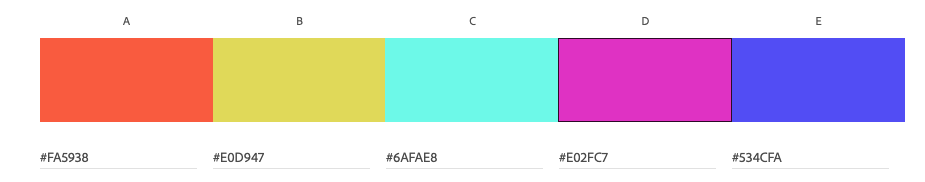
\includegraphics[width=1.0\textwidth]{images/paleta_de_cores_acessiveis.png}
        \caption{Exemplo de uma paleta de cores acessível feita no \textit{Adobe Color}}
\end{figure}  
 
\vspace*{50px}
É de extrema importância verificar como ficaria essas cores pela visão de pessoas que possuem algum tipo de daltonismo. Ao perceber que a paleta de cores ainda está com um contraste aceitável e de no mínimo 7:1 ela está pronta para o uso. 
 \begin{figure}[ht]
        \centering
    	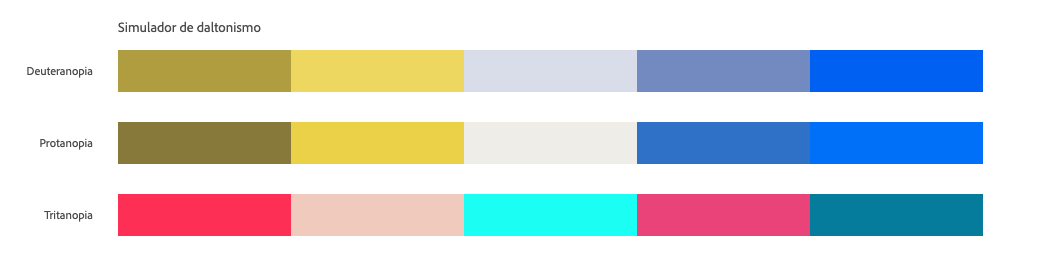
\includegraphics[width=1.0\textwidth]{images/paleta_daltonismo.png}
        \caption{simulação de daltonismo feita no \textit{Adobe Color}}
\end{figure}  


\newpage
Tipografia: A tipografia não é apenas escolher uma fonte legal para o seu projeto, junto com ela devemos levar em consideração vários aspectos que são importantes e foram listados nas diretrizes: 
\begin{itemize}
\item Espaçamento
\begin{itemize}
\item O espaçamento deve ser bem planejado para que seja possível aplicar um zoom de 200\%\ e ou ainda em caso de redimensionamento de tela o texto deve permanecer legível. 
\end{itemize}
\item Altura de linhas
\begin{itemize}
\item Sempre que houver um redimensionamento os textos não devem perder legibilidade.
\end{itemize}
\item Hierarquia tipográfica
\begin{itemize}
\item Sempre que o conteúdo da tela for dividido em sessões, todas devem possuir títulos claros, com níveis de hierarquia bem definidos, para assim manter a hierarquia da informação de uma forma concisa. 
\end{itemize}
\item Pesos, cores e contraste. 
\begin{itemize}
\item O contraste entre textos e telas também deve ser mantido num padrão de no mínimo 4:5:1
\end{itemize}
\end{itemize}

\begin{figure}[ht]
        \centering
    	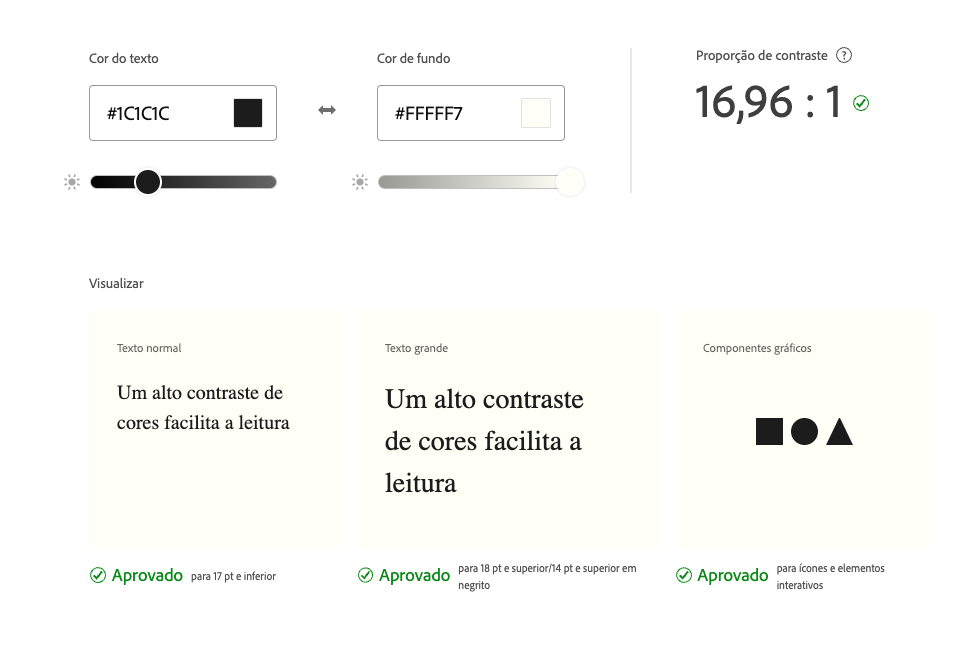
\includegraphics[width=1.0\textwidth]{images/contrast_check.png}
        \caption{Checagem do contraste de textos e fundo no \textit{Adobe Color}}
\end{figure} 

\newpage
Elementos de UI: Aqui sempre será listado e exemplificado cada elemento que vai compor a UI. Na construção desses elementos é feito o detalhamento visual, ou seja, os tamanhos, espaços, margens, cores que ele deve possuir como também os seus estados comportamentais, se houver um erro como ele se comporta, em caso de elemento focado como deve ficar o elemento.

\begin{wrapfigure}{l}{0.5\textwidth}
        \begin{center}
    	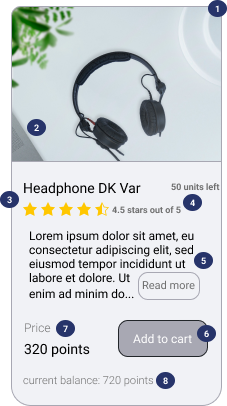
\includegraphics[width=0.48\textwidth]{images/ui-exemplo.png}
        
        \end{center}
        \caption{Exemplo de um componente montado com elementos de UI}
\end{wrapfigure} 

Com o componente \textit{Card} do exemplo ao lado podemos analisar onde as diretrizes foram aplicadas e como elas impactam na construção de componentes mais complexos de UI. 
\begin{itemize}
\item O elemento sinalizado como 1 está recebendo foco (diretriz 3.2.1 e 2.4.7), a arquitetura desse elemento está fazendo sentido para todos, sejam ouvintes ou leitores (diretriz 1.3.1). A apresentação das informações segue uma sequencia lógica (diretriz 1.3.2).  
\item O número 2 refere-se a imagem onde ela deve ter uma descrição alternativa em texto (diretriz 1.1.1) e deve ter um contraste não textual (diretriz 1.4.11).
\item O terceiro item compreende o cabeçalho do Card. Nesse cabeçalho deve haver um contraste textual de no mínimo (diretriz 1.4.3) e esse cabeçalho deve ser claro o suficiente para a finalidade do conteúdo (diretriz 2.4.6).
\item O quarto item compreende a informações adicionais, sejam elas quantos itens restam disponíveis para compra ou a avaliação daquele item. Para essas informações adicionais além de estarem descritas de forma não "convencional" aos padrões usuais de \textit{e-commerce} foram aplicadas as diretrizes de contraste textual (diretriz 1.4.11), contraste melhorado (diretriz 1.4.6), etc.
\end{itemize}
\newpage
\begin{itemize}
\item O quinto item é a descrição do produto, essa descrição não está exposta em sua totalidade, para ler o texto completo é necessário apertar o botão para ler mais. Além de todas as diretrizes de contraste que foram aplicadas, está sendo usado as diretrizes de foco (diretrizes 2.4.7 e 3.2.1), o botão presente segue a diretriz de tamanho de área clicável (diretriz 2.5.5), além de ter o nome acessível (diretriz 2.5.3). No botão em questão ainda há o acionamento e foco por teclado (diretrizes 1.4.12, 1.4.13, 2.1.1, 2.1.2 e 2.1.3). 
\item O botão sinalizado pelo número 6 segue as mesmas diretrizes do botão listado no item 5. Além das diretrizes relacionadas a foco (diretriz 2.4.3, 2.4.7), navegação (diretriz 3.2.3, 1.4.12, 1.4.13, 2.1.1, 2.1.2 e 2.1.3), localização (diretriz 2.4.8, 3.2.4) e acionamento (diretriz 2.5.2).
\item O item 7 refere-se a informações sobre preços, onde há um contraste muito nítido para evidenciar a informação mais importante, que no caso é o valor. Nesse item contempla todas as diretrizes de contraste. 
\item O item 8 é uma abordagem diferenciada para informações que são úteis em contextos gerais. Nesse caso é muito atrativo para usuários ouvintes saberem sempre quanto pontos eles dispõem em sua conta, então essa informação está disposta mais facilmente. 
\end{itemize}

}

\subsection{Fase 2: Adaptação e construção da UI acessível e usável usando o guia de acessibilidade e \textit{style guide}}
{A segunda fase se concentrou na adaptação da UI e na construção de novos componentes para o \textit{e-commerce}, sempre seguindo os guias. Nessa fase o foco principal se dividiu em duas vertentes:
\begin{itemize}
\item Criar abordagens inteligentes para problemas de acessibilidade em imagens, formulários e navegação e a adaptação de componentes com \textit{HTML} não semântico para semântico.
\item  Adaptar e criar componentes para que as tecnologias assistivas pudessem entendê-los corretamente e assim ter uma a navegação por teclado eficaz.

\end{itemize}
}
\subsubsection{Abordagens inteligentes e adaptação de componentes}
{\begin{itemize}
    \item O primeiro passo a se fazer foi organizar o \textit{HTML} de forma logica e semântica, onde cada tag \textit{HTML} deve ser usada para o fim que ela foi criada seguindo uma ordem que seja compreensível além de corresponder ao conteúdo desejado. Nesse ponto em um sistema legado muitos componentes estavam escritos de maneira errada, algumas tags \textit{HTML} estavam sendo usadas com um proposito diferente do que ela foi criada e para esses casos utilizamos a abordagem \textit{WAI-ARIA} para que o leitor conseguisse entender o que era cada tag daquela e também fosse possível fazer a navegação via teclado.

\newpage

{\textbf{Caso de uso 1:} Adaptação de um botão que foi construído de forma não acessível e por isso não era lido por leitores de tela e nem navegável via teclado. Nesse exemplo, foi usado o atributo role do \textit{WAI-ARIA} para dar o comportamento de botão a essa \lstinline{div} e com isso ganhar todos os atributos que um botão teria.

\begin{lstlisting}[language=html, caption=Componente de botão antes de receber boas praticas e acessibilidade]
    <div
        className="button__add"
        onClick={event => onClick(event)}
    >
      Adicionar ao carrinho 
    </div>
\end{lstlisting}}
{\begin{lstlisting}[language=html,caption=Adaptação do componente de botão usando \textit{WAI-ARIA}]
<div 
    role="button" 
    tabIndex="0" 
    className="button__add"
    onClick={event => onClick(event)}
    onKeyDown={event => keyHandler(event, props.onClick)}
    {...props}
>
    Adicionar ao carrinho
</div>
 
\end{lstlisting}}

\vspace*{50px}
{\textbf{Caso de uso 2:} Adaptação e construção de imagens acessíveis. 
\item As imagens que possuem algum tipo de conteúdo devem ser acessíveis, elas precisam de alguma descrição, seja ela visível ou não. Existe o atributo \lstinline{alt} para a \textit{tag} \lstinline{img}, onde ele serve para descrever o que está presente na imagem. Essa descrição do \lstinline{alt} não aparece visualmente, mas ela é lida pelo leitor de tela, quando o usuário, navegando pelo teclado, passar pela imagem.}
{\begin{lstlisting}[language=html,caption=usando atributo alt]
<img src="headphone.jpg" alt="Headphone na cor preto"> 
\end{lstlisting}}
\item Caso haja necessidade de fornecer uma informação contextualizada é necessário fazer uso do atributo \lstinline{title}. Nesse caso, a maioria dos leitores de tela lerá o texto alternativo, o atributo de título e o nome do arquivo. Além disso, os navegadores exibem o texto do título como dicas de ferramentas quando estão sobre o mouse. Com a chegada do \textit{HTML 5} surgiram dois novos elementos o \lstinline{<figure>} e \lstinline{figcaption>}, que devem associar uma figura a uma legenda. 
{\begin{lstlisting}[language=html,caption=usando atributo alt]
<figure>
  <img src="headphone.jpg" alt="Headphone na cor preto"> 
  <figcaption>Headphone com microfone acoplado na cor preta, com um fio de ótima construção</figcaption>
</figure>
\end{lstlisting}}

\item  Ainda temos os casos onde as imagens são apenas decorativas e como elas não carregam conteúdo elas devem ser ignoradas pelos recursos de tecnologia assistivas. Para esse caso nós temos três tipos de abordagens: 
\begin{itemize}
\item Por ser decorativa a melhor abordagem é incluí-las na página como imagens de fundo através de \textit{CSS} E caso a imagem transmita significado ao conteúdo, mas tenha sido inserida via \textit{CSS}, pode-se utilizar recursos \textit{WAI-ARIA}.
{\begin{lstlisting}[language=html,caption=adicionando imagem via CSS]
<style>
div {
    background-image:url("./images/headphone-preto.png");
}
</style>
\end{lstlisting}}
\item Em casos de imagens que usam a \textit{tag} \lstinline{img} basta ter uma descrição \lstinline{alt} vazia. Isso é para fazer com que os leitores de tela reconheçam a imagem, mas não tentem descrever a imagem. A razão para usar um \lstinline{alt} vazio ao invés de não incluí-lo é porque muitos leitores de tela anunciam o URL da imagem inteira se nenhum \lstinline{alt} for fornecido.
{\begin{lstlisting}[language=html,caption=usando atributo alt vazio]
<img src="logotipo.jpg" alt=""> 
\end{lstlisting}}

\item Em casos de imagens incluídas em tags que não são \lstinline{img} podemos fazer uso o atributo \textit{ARIA role} \lstinline{(role="presentation")}, isso também impede que os leitores de telas leiam textos alternativos.
{\begin{lstlisting}[language=html,caption=usando atributo rele="presentation"]
<div role="presentation" src="logotipo.jpg" alt="" />
\end{lstlisting}}
\end{itemize}


 
\end{itemize}}

{
\textbf{Caso de uso 3:} Criando formulários acessíveis.

\begin{itemize}
    \item O primeiro passo para criar um formulário acessível é criar uma estrutura \textit{HTML} com sequência lógica, essa sequencia é definida pela ordem que se encontra o \textit{HTML}. Fazendo isso a navegação pelos campos do formulário ficará mais fácil tanto por teclado quanto para leitores de tela. 
    \item Sempre associe um campo de entrada a um rótulo. E quando não for possível fazer essa associação por tags \textit{HTML} faça via \textit{WAI-ARIA} usando o atributo \lstinline{aria-label}.
    \item Forneça sempre instruções claras sobre os dados de entradas pedidos no campo. As entradas devem ser facilitadas, retire caracteres especiais em campos numéricos e etc. 
    \begin{itemize}
        \item Para campos com obrigatoriedade de dados, deve-se ter um indicador visual e escrito de obrigatoriedade. O atributo \lstinline{required} auxilia no quesito de obrigatoriedade de um campo.
        \item Podemos adicionar também o atributo de estado \lstinline{aria-invalid} que pode ter os valores \textit{true} ou \textit{false} para indicar se o campo está válido ou inválido.
    \end{itemize}
    \item Sempre identifique e descrever erros de entrada de dados e confirmar o envio de informações para o usuário. 
    \begin{itemize}
        \item A indicação do erro é feita de três formas: com uma cor, um texto informativo e um ícone de alerta. Assim, não usamos somente uma forma para representar esta informação, beneficiando pessoas sem deficiência visual, com deficiências cognitivas, que usam leitor de telas ou que possuem daltonismo;
        \item Adicione um área para mensagem informativa de forma geral do formulário e uma área de mensagem abaixo de cada campo com erro. Esta área de mensagem informativa do formulário possui os atributos \lstinline{role="alert"}, que avisa que é uma mensagem de alerta e \lstinline{aria-live="assertive"} que informa que é um campo que pode sofrer modificações no conteúdo e o leitor de telas é informado quando há modificação neste campo;
    \end{itemize}
    \item Aplique distinção visual de qual campo está recebendo o foco no momento, mesmo aplicando o \lstinline{outline} padrão do navegador. A customização desse \lstinline{outline} pode ser feita para que ele sempre fique visível qual campo contém o foco.
    
    {\begin{lstlisting}[language=html, caption=Formulário acessível]
    <form>
        <output id="formMessage" role="alert" aria-live="assertive" tabindex="0" class="error">
            O formulário apresenta erros que impedem a finalização do seu cadastro. Confira se todos os campos obrigatórios foram preenchidos e tente novamente.
        </output>

        <p>
            <label for="email1">
                E-mail <span class="required">(obrigatório)</span>:
            </label>
            <input type="email1" name="email1" id="email1" required="" aria-invalid="true" aria-describedby="emailMessage">
            <span class="fieldMessage" id="emailMessage">
                O e-mail não pode ficar em branco e deve ser válido.
            </span>
          </p>
  
          <p>
            <label for="phone1">
                Telefone <span class="optional">(opcional)</span>:
            </label>
            <input type="tel" name="phone1" id="phone1" aria-describedby="phoneTip">
            <span class="fieldTip" id="phoneTip">
                Formato: (99) 99999-9999.
            </span>
          </p>

        <button class="formButton" id="formButtonARIA" type="submit">Finalizar cadastro</button>
    </form>
    \end{lstlisting}}
    
    \begin{figure}[ht]
  		\center
        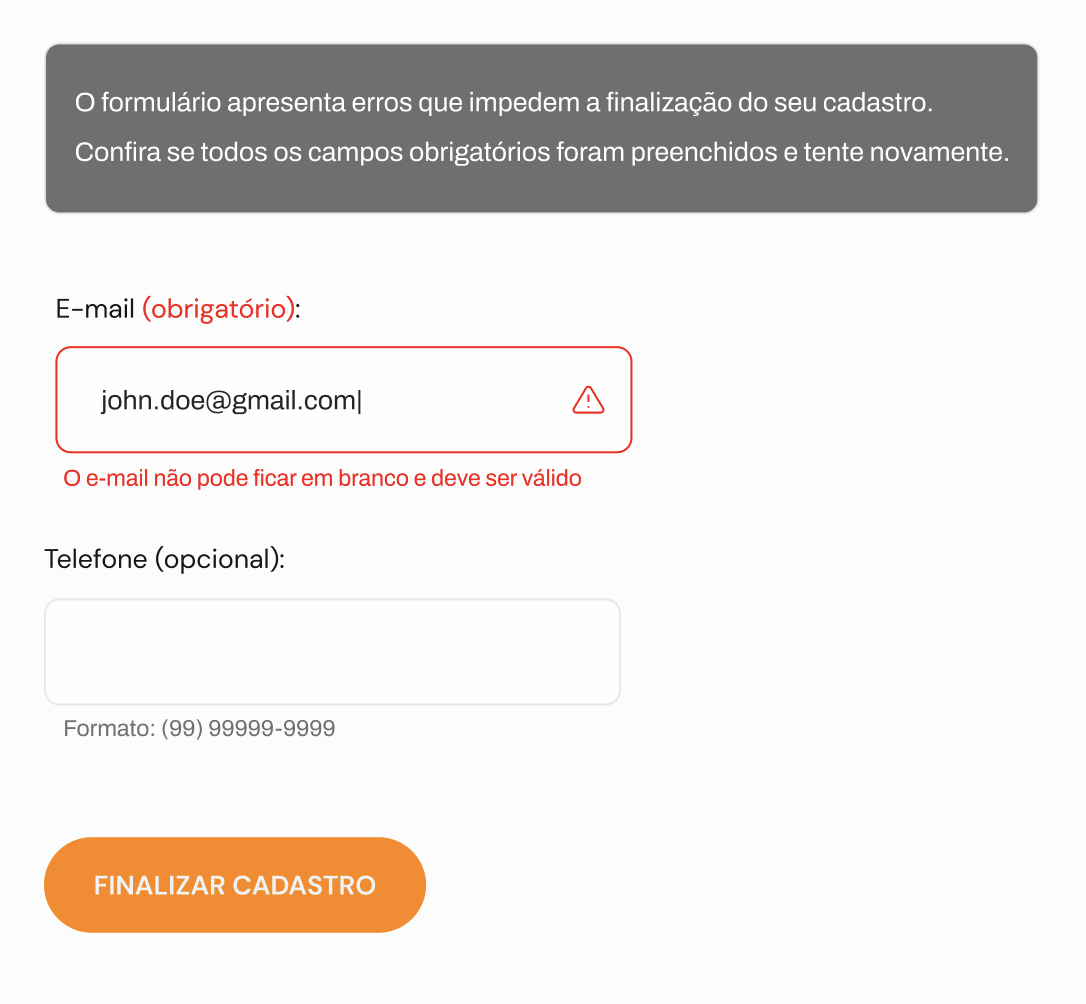
\includegraphics[width=0.7\textwidth]{images/form-acessivel.png}
        \caption{Formulário criado usando as técnicas listadas acima}
    \end{figure} 
\end{itemize}
}
\subsubsection{Adaptação de componentes para o uso de leitores de telas e navegação por teclado}
{Antes de falar de adaptação de componentes é necessário entender como funciona o leitor de telas. O leitor de telas basicamente é um software que vai percorrendo textos e imagens e lendo em voz alta tudo o que ele encontra na tela, a partir do momento que o usuário começa a interagir com o software para efetuar uma navegação ele vai percorrendo o documento saltando entre elementos interativos e cabeçalhos.Para que essa navegação ocorra deve está tudo funcionando direito, pois caso contrário o usuário pode se perder na página e ter dificuldades em entender como a informação está organizada. No leitor de telas a navegação ocorre de três maneiras: 
\begin{itemize}
    \item Navegação com as setas direcionais: Usando a navegação por setas direcionais o usuário consegue acessar as informações textuais.
    \item Navegação por tecla \textit{tab}: O leitor sai pulando para os links espalhados na página.
    \item Navegação com a tecla h: O leitor salta entre os cabeçalhos marcados na página.
\end{itemize}

\newpage

{\textbf{Caso de uso 1:} Navegação por cabeçalhos.

Cabeçalhos compõem a hierarquia de informação do site, essa hierarquia é usada pelos leitores de tela para navegação dentro da página. A grande maioria dos leitores de tela dispõem de atalhos para acesso rápido aos cabeçalhos marcados na página. Para garantir que tecnologias assistivas acessem o conteúdo dos cabeçalho sem sua ordem de importância é preciso tomar alguns cuidados: 
\begin{itemize}
    \item Cuidado com múltiplas \textit{tags} \lstinline{h1} na página. Mesmo que haja separação de contexto para a utilização de mais de um \lstinline{h1} por página o leitor de tela não consegue identificar a diferença e a importância de \lstinline{h1} contidos em outras \textit{tags}.
    \item Para essa navegação funcionar, o código precisa ter sido escrito com a semântica correta, ou seja, cabeçalhos devem ser definidos como cabeçalhos e não usar qualquer outro artificio visual para se assemelhar a um cabeçalho. 
\end{itemize}
{\begin{lstlisting}[language=html,caption=cabeçalhos com hierarquia]
<h1>Cabeçalho Principal</h1>
<p>Exemplo de um texto de um parágrafo</p>
<h2>Cabeçalho Secundário</h2>
<p>Mais texto de um parágrafo.</p>
\end{lstlisting}}


{\textbf{Caso de uso 2:} Navegação por tabulação e leitores de tela.

A ordem da navegação por tabulação é derivada da forma como o \textit{layout} do \textit{site} está escrito, contudo a ordem padrão pode não corresponder necessariamente a ordem visual. Ao utilizar a tecla \textit{tab}, o leitor de tela realiza o foco e lê em voz alta os links e componentes interativos presentes na página.  A tabulação é utilizada somente para navegar entre os links, e com isso todos os links terão que ser localizados através destas duas formas, com a tabulação ou com as setas. O que diferencia uma forma da outra, é que com as setas, o usuário poderá ler toda a página (incluindo texto entre os links), e com a tabulação, o usuário só pode localizar os links, botões, campos de edição, e caixas de seleção.


Navegar por entre os links é uma forma de observar o texto rapidamente, especialmente se os usuários estiverem tentando encontrar uma seção específica do \textit{website}. Para ter uma navegação por tabulação eficiente é preciso passar por alguns pontos: 
\begin{enumerate}
    \item Ordene de forma lógica e intuitiva a leitura e tabulação. Preparar o \textit{HTML} para ter uma navegação consistente e eficaz é essencial para o bom funcionamento da navegação atrelada a leitores de tela. 
    \item Usar a tecla \textit{tab} para passar pelos links e controles de formulários
    das páginas, certificando-se de que todos os links e controles de
    formulários podem ser acessados, bem como se os links indicam
    claramente para onde levam. 
    \begin{itemize}
        \item Com atributo \lstinline{tabindex} é possível definir uma ordem de foco nos elementos dispostos na tela. Usando o \lstinline{tabindex=0} é inserido um elemento na ordem natural de tabulação e com \lstinline{tabindex="-1"} um elemento é removido da ordem e tabulação.
        \newpage
{\begin{lstlisting}[language=html,caption=Uso do atributo tabindex]
<label>
    Primeiro na lista de tabulação:<input type="text">
</label>
<div tabindex="0">
Próximo item na lista de tabulação, mesmo não sendo um elemento que receberia o foco natural
</div>
<div>Não será focado pois está sem o tabindex</div>
\end{lstlisting}}
        \item Adicione o atributo \lstinline{title} aos links, ele mostrará uma descrição do lugar pra onde o link leva, melhorando a navegação.
{\begin{lstlisting}[language=html,caption=usando o atributo title]
<a href="#" onclick="abrePopup()" onkeypress="abrePopup()" title="Abre uma janela pop-up com Javascript">Ver mais informações</a>
\end{lstlisting}}
    \end{itemize}
    \item Forneça âncoras para ir direto a um bloco de conteúdo. São comumente chamados de \textit{landmarks} é um tipo de região em uma página web a qual uma pessoa pode querer acessá-la rapidamente. Um dos principais benefícios em se usar pontos de referência é a possibilidade de o usuário acessar diretamente uma região da página sem a necessidade de seguir a ordem natural do conteúdo. Isso é especialmente relevante para o caso de pessoas que utilizam leitores de tela para navegar na \textit{Web}. Para essa abordagem é muito utilizado o CSS deixando-os links invisíveis e apenas disponíveis quando a navegação por tabulação se iniciar. 
{\begin{lstlisting}[language=html,caption=usando landmarks]
<div role="heading" id="cabecalho"> 
  <h1>O Cabeçalho</h1> 
  <a href="#conteudo" accesskey="p">Pular para o conteúdo principals</a> 
</div> 
<div role="navigation" id="navegacao"> conteúdo da navegação </div>
<div role="main" id="conteudo"> conteúdo da main </mdiv>
\end{lstlisting}}
    \item Não utilize tabelas para diagramação. As tabelas devem ser utilizadas apenas para dados tabulares e não para efeitos de disposição dos elementos na página. O leitor de telas sairá pulando por cada campo das tabelas e o usuário poderá ficar perdido na navegação. Para efeitos de diagramação faça uso de \textit{CSS}.
    \item Separe os links adjacentes. Em uma sequência de links, além do espaço, é importante o uso de separadores ou elementos do HTML adequados para que as pessoas com deficiência identifiquem claramente onde termina e começa um novo link. É recomendado o uso de listas , em que cada elemento dentro da lista é um link.
{\begin{lstlisting}[language=html,caption=separando links adjacentes]
<ul id="menu">
    <li> <a href="home.html">Home</a></li>
    <li> <a href="pesquisa.html">Pesquisa</a></li>
</ul>
\end{lstlisting}}
    \item Não abrir novas instâncias sem a solicitação do usuário. Não use o redirecionamento automático de páginas. Forçar a abertura de links em uma nova janela não é algo esperado e o usuário se perderá na navegação. Caso implemente essa funcionalidade, o link deve possuir uma iconografia óbvia e explicativa, usando pseudo-elemento \lstinline{::after} no CSS. Lembre-se que em CSS, o conteúdo em pseudo-elementos é lido em voz alta por leitores de tela. Certifique-se de que contém informações relevantes.
    \item Garanta que o conteúdo possua o foco por mouse ou teclado. Esse foco deve ser visível. Para pessoas com baixa visão, é muito importante que seja possível perceber facilmente onde está o foco do teclado, garantindo uma maior facilidade de navegação. A pseudo-classe \lstinline{:focus} é utilizada para definir o estilo de qualquer elemento HTML que receber o foco do teclado, como links e elementos de formulário.
{\begin{lstlisting}[language=html,caption=usando o foco visível]
a:focus, a:hover {
    border: 2px solid #F00;
}
\end{lstlisting}}
    \item Garanta que todas as funcionalidades que estão disponíveis via mouse também estarão disponíveis para serem acionadas via teclado. Só dessa forma o site estará totalmente acessível para pessoas com deficiências. 
\end{enumerate}
}
}
}

\subsection{Fase 3: Construção do dashboard acessível}
{Para a construção do \textit{dashboad} com gráficos foi utilizado a biblioteca D3.js que é usada para visualização de informação. Essa biblioteca permite que seja construído aplicações em que os dados entram puros e são dinamicamente associados em representações gráficas. Com o D3 o DOM (Document Object Model) pode ser facilmente manipulado já que ele usa usa os padrões da web como HTML, CSS, SVG para renderizar gráficos de visualização poderosos.}

{\textbf{Construção de gráficos com D3.js:}

Para manipularmos o DOM (Document Object Model), precisamos aprender a utilizar os recursos presente no D3. O D3 usa JavaScript para realizar a maioria das tarefas de seleção, transição e vinculação de dados.

{\textcolor{blue}{OPTAMOS POR NAO CONSTRUIR O GRAFICO TODO COM D3 E SIM APENAS AS PARTES QUE ERAM NECESSÁRIAS PARA EVITAR ENGASGOS DE PERFORMANCE. Entao era feito o esqueleto em html e adicionado as tags necessarias via d3.}}

A primeira coisa necessária para construir um gráfico com D3.js é adicionar a biblioteca ao projeto, seja por gerenciador de pacotes ou por importação direta na tag \lstinline{script}. Feito isso, é preciso ter uma tag como base onde as partes do gráfico serão injetadas, geralmente é usada a tag \lstinline{svg} pois ela auxilia na construção de formas geométricas que será utilizado no gráfico.

}
\subsection{Fase 4: Testes e avaliações de acessibilidade}
{Durante e após a construção do e-commerce de acordo com os
padrões Web e as diretrizes de acessibilidade, é necessário efetuar testes para garantir sua acessibilidade. Esses testes foram executados de dois modos: 
\begin{itemize}
\item Avaliação automática: São as avaliações feitas de maneira automática por meio de \textit{plugins} de verificação e de \textit{websites} de validação.
\begin{itemize}
\item \textit{Google Accessibility Developer Tools} ({Plugins} para navegador \textit{Chrome}).
\item \textit{DevTools }({Plugins} para navegador \textit{Chrome}).
\item Contrast Checker (website - Validação de contraste de cores
\end{itemize}
\item Avaliações manuais: Essa etapa pode ser feita usando o leitor de tela e a navegação por teclado, onde deve ser checado se todos os comportamentos e ações esperados estão sendo realmente respeitados e executados. 
\end{itemize}
}

\subsection{Tecnologias utilizadas} 
{A linguagem de programação JavaScript foi escolhida para a elaboração deste trabalho devido a sua grande relevância no frontend. Entre as principais bibliotecas utilizadas neste projeto destaca-se:
\begin{itemize}
\item \textit{HTML}(é uma linguagem de marcação utilizada na construção de páginas na \textit{Web}).
\item Diretrizes \textit{WCAG} (definem a forma de como tornar o conteúdo da \textit{Web} mais acessível para pessoas com deficiência).
\item \textit{WAI-ARIA} (Oferece maneiras de tornar as aplicações mais acessíveis a uma diversidade maior de pessoas, incluindo quem utiliza tecnologias assistivas, como leitores de telas).
\item React.js (É uma biblioteca \textit{JavaScript} para criar interfaces de usuário, ela é declarativa e baseada em componentes)
\item Sass ( \textit{Syntactically Awesome Style Sheets} é uma linguagem de extensão do \textit{CSS}, tem como objetivo tornar o processo de desenvolvimento mais simples e eficiente)
\item D3.js (é uma biblioteca {JavaScript} para construção de visualizações de dados. \textit{D3} permite que visualizações sejam criadas diretamente em páginas \textit{HTML} através de gráficos vetorizados \lstinline{SVG}).
\item Tecnologias assistivas:
\begin{itemize}
\item VoiceOver
\item NVDA
\item ORCA
\end{itemize}
\end{itemize}
 }
\subsection{Contribuição}
{⁠A solução ainda não se encontra em ambiente de produção, pois está passando por um processo de alinhamento sobre outros pontos que o cliente deseja modificar dentro do sistema. Entretanto, todo esse épico de acessibilidade e DataViz já foi aprovado e muito bem avaliado pelo cliente que se mostrou muito feliz com o que foi apresentado.

Esse projeto e tudo construído nele se tornou um tipo de referência para outros desenvolvedores e designers que buscam aprender mais sobre a acessibilidade e aplicá-la de um modo descomplicado e correto, o guia está sendo construído justamente com a intenção de ser um objeto compartilhado pelos desenvolvedores do CESAR e servir como orientação para todos. 

}
